\documentclass[twoside]{article}
\setlength{\oddsidemargin}{-0.5 in}
\setlength{\evensidemargin}{1.5 in}
\setlength{\topmargin}{-0.6 in}
\setlength{\textwidth}{5.5 in}
\setlength{\textheight}{8.5 in}
\setlength{\headsep}{0.5 in}
\setlength{\parindent}{0 in}
\setlength{\parskip}{0.07 in}
\setlength{\marginparwidth}{145pt}

%
% ADD PACKAGES here:
% 12

\usepackage{amsmath,
            amsfonts,
            amssymb,
            graphicx,
            mathtools,
            flexisym,
            marginnote,
            hyperref,
            titlesec}

\usepackage[english]{babel}
\usepackage[utf8]{inputenc}
\usepackage[shortlabels]{enumitem}

\graphicspath{ {images/} }

\hypersetup{
    colorlinks=true,
    linkcolor=blue,
    filecolor=magenta,      
    urlcolor=blue,
}

\titlespacing\section{0pt}{12pt plus 4pt minus 2pt}{0pt plus 2pt minus 2pt}
\titlespacing\subsection{0pt}{12pt plus 4pt minus 2pt}{0pt plus 2pt minus 2pt}

%
% The following commands set up the lecnum (lecture number)
% counter and make various numbering schemes work relative
% to the lecture number.
%
\newcounter{lecnum}
\renewcommand{\thepage}{\thelecnum-\arabic{page}}
\renewcommand{\thesection}{\thelecnum.\arabic{section}}
\renewcommand{\theequation}{\thelecnum.\arabic{equation}}
\renewcommand{\thefigure}{\thelecnum.\arabic{figure}}
\renewcommand{\thetable}{\thelecnum.\arabic{table}}

\newcommand{\aosv}{1044414: Advanced Operating Systems and Virtualization}
\newcommand{\wir}{1038137: Web Information Retrieval}
\newcommand{\va}{1052057: Visual Analytics}
\newcommand{\advprog}{1044416: Advanced Programming}
\newcommand{\dchpc}{1044399: Data Centers and High Perf. Computing}

\newcommand{\qu}[1]{\marginnote{\textcolor{cyan}{#1}}}


%
% The following macro is used to generate the header.
%
\newcommand{\lecture}[4]{
   \pagestyle{myheadings}
   \thispagestyle{plain}
   \newpage
   \setcounter{lecnum}{#4}
   \setcounter{page}{1}
   \noindent
   \begin{center}
   \framebox{
      \vbox{\vspace{2mm}
    \hbox to 7.4in { {\bf #1
    \hfill Spring 2018} }
       \vspace{4mm}
       \hbox to 7.4in { {\Large \hfill Lecture #4: #2  \hfill} }
       \vspace{2mm}
       \hbox to 7.4in { {\it Lecturer: #3 \hfill Scribe: Anxhelo Xhebraj} }
      \vspace{2mm}}
   }
   \end{center}
   \markboth{Lecture #4: #2}{Lecture #4: #2}

   \iffalse
   {\bf Note}: {\it LaTeX template courtesy of UC Berkeley EECS dept.}

   {\bf Disclaimer}: {\it These notes have not been subjected to the
   usual scrutiny reserved for formal publications.  They may be distributed
   outside this class only with the permission of the Instructor.}
   \vspace*{4mm}
   \fi
}
%
% Convention for citations is authors' initials followed by the year.
% For example, to cite a paper by Leighton and Maggs you would type
% \cite{LM89}, and to cite a paper by Strassen you would type \cite{S69}.
% (To avoid bibliography problems, for now we redefine the \cite command.)
% Also commands that create a suitable format for the reference list.
\iffalse
\renewcommand{\cite}[1]{[#1]}
\def\beginrefs{\begin{list}%
        {[\arabic{equation}]}{\usecounter{equation}
         \setlength{\leftmargin}{2.0truecm}\setlength{\labelsep}{0.4truecm}%
         \setlength{\labelwidth}{1.6truecm}}}
\def\endrefs{\end{list}}
\def\bibentry#1{\item[\hbox{[#1]}]}
\fi

%Use this command for a figure; it puts a figure in wherever you want it.
%usage: \fig{NUMBER}{SPACE-IN-INCHES}{CAPTION}
\newcommand{\fig}[3]{
            \vspace{#2}
            \begin{center}
            Figure \thelecnum.#1:~#3
            \end{center}
    }
% Use these for theorems, lemmas, proofs, etc.
\newtheorem{theorem}{Theorem}[lecnum]
\newtheorem{lemma}[theorem]{Lemma}
\newtheorem{proposition}[theorem]{Proposition}
\newtheorem{claim}[theorem]{Claim}
\newtheorem{corollary}[theorem]{Corollary}
\newtheorem{definition}[theorem]{Definition}
\newenvironment{proof}{{\bf Proof:}}{\hfill\rule{2mm}{2mm}}

% **** IF YOU WANT TO DEFINE ADDITIONAL MACROS FOR YOURSELF, PUT THEM HERE:

\newcommand\E{\mathbb{E}}

\begin{document}

\nocite{*}

%FILL IN THE RIGHT INFO.
%\lecture{**LECTURE-NUMBER**}{**DATE**}{**LECTURER**}{**SCRIBE**}

\lecture{\aosv}{March 2}{Alessandro Pellegrini}{1}

%\footnotetext{These notes are partially based on those of Nigel Mansell.}

% **** YOUR NOTES GO HERE:
\section{Course Information}
\subsection{Exam}
The exam is composed of two parts:
\marginnote{\href{https://www.diag.uniroma1.it/~pellegrini/didattica/2017/aosv/0.Introduction.pdf}{Slides 0.}}
\begin{itemize}
  \item $[2/5]$ \textbf{Written Part}: 3 theoretical or practical questions
  \item $[3/5]$ \textbf{Practical Project}: same project for everyone to be done singularily. Specifications will be given in the in the middle of the course
\end{itemize}
The two parts must be done within one year from each other.
In the course we will see various versions of the Linux kernel (2.4, 3.0, 4.0). Any version can be used for the project. The more compatible the project is with the various versions, the better.
\subsection{Course outline}
In this course we will try to understand the internals of an operating system. \marginnote{Slides 0. - pp. 4} We will use the Linux kernel as reference since it is open source and permits to get some good hands-on experience to understand basic principles that are applied to all operating systems in general.

Regarding the architecture during the course we will use the Intel architecture as reference.

We will see how to develop kernel modules, to perform kernel debugging and hot patching.

\section{Boot Sequence}
After hitting the powerup button the Boot Sequence starts. It is composed of 6 levels:
\begin{description}
  \itemsep0em 
  \item[BIOS] (Basic Input Output System) code stored in flash ROM inside the motherboard to check what hardware devices are connected to the system etc. It calculates how much RAM is available and performs some consistency checks. It creates a memory map and a map of all devices installed in the system. \marginnote{ACPI Table: describes what peripherals are installed in the system}[- 36pt]
  Finally the BIOS loads the Bootloader.

  Since BIOS became very convoluted over years a new specification was developed: \href{https://en.wikipedia.org/wiki/Unified_Extensible_Firmware_Interface}{\textbf{UEFI}} (Unified Extensible Firmware Interface). UEFI is a tentative of replacing the BIOS firmware interface to give more programming versatility and other features (even security wise).
  \item[Bootloader Stage 1] It searches among the various devices to load the Bootloader Stage 2. This is done because BS1 does not have enough space to load the system (less than 512 Bytes in length).
  \item[Bootloader Stage 2] loads from the storage the kernel image and executes it. 

  \newpage

  \item[Kernel Startup] is performed between two levels: hardware interaction through assembly code and internal data structures initialization. Spawns the first process: Init.

  \item[Init] Its goal is to startup and configure the environment known as Runlevels/Targets: Desktop Environment etc.
  
  \item[Runlevels/Targets] subset of services to be executed on startup.
\end{description}

\section{x86 Initial Booting Sequence}
Intel processors work on different voltage levels and in order to work 3 reference voltages (3.3V, 5V, 12V) called \textbf{rails} must be supplied by the Power Supply Unit (PSU). In addition, voltage regulators on the motherboard or in other components convert these standard voltages to others as necessary (for example DDR2 and DDR3 dual inline memory modules (DIMM) require 1.8 V and 1.5 V). After completing internal tests and determining that the power is ready for use the PSU triggers the Power Good signal informing the motherboard \cite{ATX,PG}.

Finally, clocks are derived from a small number of input clocks and oscillator sources and the reset signal is triggered which gives control to the BIOS.

\subsection{Real Mode}
One \marginnote{\href{https://www.diag.uniroma1.it/~pellegrini/didattica/2017/aosv/1.Initial-Boot-Sequence.pdf}{Slides 1.}} CPU is dynamically chosen to be the bootstrap processor (BSP) that runs all of the BIOS and kernel initialization code. The remaining processors, called application processors (AP) at this point remain halted until later. In this primitive power up state the processor is in \textbf{real mode} with memory paging disabled (Paging unit disabled) behaving like the original 1978 Intel 8086. In this mode memory is accessed through \textit{Segmentation-based addressing}. The wrangling of the adresses is managed by the \textbf{Segmentation Unit} that transforms \textbf{Logical Adresses} into \textbf{Linear Adresses} (which coincides with the Physical Address in real mode).
\begin{center}
  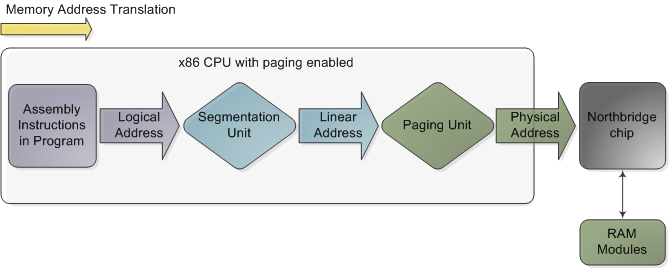
\includegraphics[width=0.8\textwidth]{memtrans.png}
  \fig{1}{0 pt}{Address Translation}
\end{center}

The \marginpar{\textsc{Segment Registers}} original 8086 processor had words of 16-bits and this allowed code to work only with $2^{16}$ bytes (64K). In order to increase addressable memory, segment registers were introduced besides general registers (\texttt{AX}, \texttt{BX} etc.) to inform the CPU in which of the chunks of memory a program's instructions were going to work on. There were four segment registers: one for the stack (\texttt{SS}), one for program code (\texttt{CS}) , and two for data (\texttt{DS}, \texttt{ES}). Nowadays \textbf{segmentation} is \textbf{still present} and is \textit{always} enabled in x86 processors for backward compatibility. For example, a jump instruction uses the code segment register (\texttt{CS}) whereas a stack push instruction uses the stack segment register (\texttt{SS}).

Segment registers store 16-bit \textbf{segment selectors} which are 16-bit numbers specifying the physical memory address for the start of a segment (this is only in the case of real mode, in protected mode things are different). In this scenario when a physical address needs to be accessed, say for example in one of the data segments, we ask for the word in segment \\ \texttt{DS} $:=$ \texttt{0x1000} with offset \texttt{AX} $:=$ \texttt{0x0012} and the address that is accessed is denoted as \texttt{DS:AX}.

Since physical address pins cost, and at the time 1 MB of memory was thought to be more than sufficient, Intel made the decision to reduce the addressable space to $2^{20}$ by accessing physical memory through the scheme \texttt{DS} $\times \ 2^4 \ + $ \texttt{AX} instead of using the concatenation of the two registers as address (20 bits, $2^{20} = 1$ MB instead of 32 bits, $2^{32} = $ 4GB).

Real mode segment starts range from 0 all the way to \texttt{0xFFFF0} (16 bytes short of 1 MB) in 16-byte increments. To these values a 16-bit offset (the logical address) between \texttt{0x0} and \texttt{0xFFFF} is added. It \marginpar{\href{https://web.archive.org/web/20130609073242/http://www.osdever.net/tutorials/rm_addressing.php?the_id=50}{A20 Line}} follows that there are multiple segment/offset combinations pointing to the same memory location, and physical addresses fall above 1MB if your segment is high enough (Memory Wrap-Around). 

\subsection{BIOS operations}

\marginnote{
  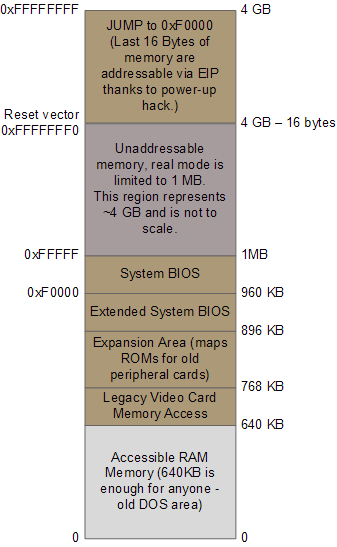
\includegraphics[scale=0.4]{bootMemReg.png}
  \fig{2}{0 pt}{Relevant Physical Memory Regions of Later x86 processors.}
  The brown regions are mapped \textbf{away} from RAM. When the processor writes/reads such regions the northbridge routes it to the right device.
}

The first operation that is fetched is processor dependent and the address at which the operation is found is called \textbf{Reset Vector}. In the case of the 8086 processor such address is \texttt{F000:FFF0} (\texttt{CS:IP}) which corresponds to the physical address $ \texttt{0xF000} \times 16 + \texttt{0xFFF0} = \texttt{0xFFFF0}$, 16 Bytes below the maximum addressable location. The 80386 CPU and later Intel processors have predefined data in some CPU registers after a computer reset: Instruction Pointer (\texttt{IP}) set to \texttt{0xFFF0}, \texttt{CS} to \texttt{0xF000} and \texttt{Base address} of the "hidden part" of the Code Segment Register set to \texttt{0xFFFF0000}. Such addresses are then used to compute the first instruction that is fetched which is \texttt{CS Base address + EIP} getting the physical address \texttt{0xFFFFFFF0} which is still 16 byte short the maximum addressable memory with 32 bits. The motherboard (Northbridge component) then ensures that the instruction at the Reset Vector is a jump to the memory location mapped to the BIOS entry point. This jump clears the hidden base address present at power up. All of these memory locations have the right contents needed by the CPU thanks to the memory map kept by the chipset. They are all mapped to flash memory containing the BIOS.

The CPU then starts executing BIOS code that initializes some of the hardware in the machine and executes \textbf{POST} code (Power-On Self Test) that tests and initializes various components in the computer. Lack of a working video card fails the POST and causes the process to halt and beep. A portion of the BIOS is dedicated for communication with legacy video cards.

After the POST the BIOS loads its configuration and then performs \textbf{Shadow RAM Initialization}: copies itself on RAM for faster access.
The last operation of the BIOS is seeking a boot device from which it loads the first 512-byte sector (sector zero/boot sector) called \textbf{Master Boot Record} to the address at \texttt{0000:7C00} and performs the jump to that address with \texttt{ljmp \$0x0000, \$0x7C00}

\subsection{Master Boot Record}
The MBR holds the code of the Bootloader Stage 1 that will load the Bootloader Stage 2.
\begin{center}
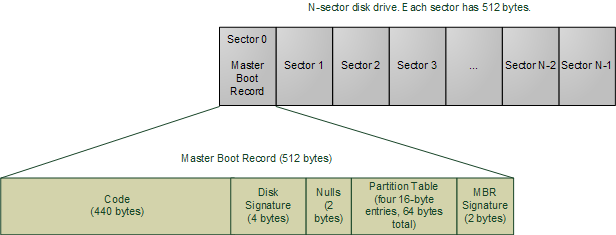
\includegraphics[width= 0.7 \textwidth]{masterBootRecord.png}
\end{center}
The partition table entries contain offsets telling the beginning of the 4 partitions. At the beginning of each partition there can be one Boot sector. To one partition entry can be designated an \textit{extended partition} which can be subdivided into a number of logical partitions. Each of the logical partitions within the extended partition is preceeded by the Extended Boot Record (EBR) and each EBR has a pointer to the next EBR forming a linked list.

The MBR Signature \textit{must be} \texttt{0x55AA}.

The initial bytes of the MBR can contain the \textbf{BIOS Parameter Block} (BPB) that is a data structure describing the physical layout of a data storage volume, in order for the BIOS to know how to read it etc. Therefore after the load another \texttt{jmp} is performed to skip the BPB.

Finally interrupts are disabled (\texttt{cli} instruction) since the stack segment is not initialized yet and all the segment selectors are set to zero to have a linear access on physical addresses.

\bibliography{Lec1}
\bibliographystyle{plainnat}
\end{document}